%-------------------------------------------------%
\documentclass[12pt,oneside]{book}
%-------------------------------------------------%
\usepackage[spanish]{babel}
\usepackage[margin=1in]{geometry}
\usepackage{graphicx}
\usepackage{amssymb,amsmath,amsthm,amsfonts}
\usepackage{enumerate}
\usepackage{lipsum}
\usepackage{color}
\usepackage{float}
\usepackage{parskip}
\usepackage{titlesec}
\usepackage{apacite}
\usepackage{hyperref}
\usepackage{changepage}
\usepackage{cite}
\usepackage{url}
\usepackage{listings}
\usepackage{color} %red, green, blue, yellow, cyan, magenta, black, white
\definecolor{mygreen}{RGB}{28,172,0} % color values Red, Green, Blue
\definecolor{mylilas}{RGB}{170,55,241}
\usepackage[framed,numbered,autolinebreaks,useliterate]{mcode}
%-------------------------------------------------%
\titleformat{\chapter}{\normalfont\huge}{\thechapter.}{20pt}{\huge \bf}
\renewcommand{\qedsymbol}{\rule{0.7em}{0.7em}}
\providecommand{\abs}[1]{\lvert#1\rvert}
\graphicspath{ {Img/} }
\decimalpoint
\newenvironment{solution}{\begin{proof}[Solución]}{\end{proof}}
%-------------------------------------------------%
\title{Tarea 3 - Optimización no Lineal}
\author{Camara Medina Cynthia Lilian \\
Reyes Zamora Ollin \\
Alanis González Edzon Omar \\
Mendoza Urrusquieta Jair Natael}
\date{\today}
%-------------------------------------------------%
\begin{document}
\maketitle
\tableofcontents
\chapter{Teoría}
\section{División de intervalos por la mitad}
Hacer cinco iteraciones a mano 1 del método de división de intervalos por la mitad, visto en clase, para acotar el mínimo del siguiente problema:
Minimizar \[f(x)=4x^2+\frac{1}{x^4}\] dentro del intervalo $[0.7,2.5]$. Reportar los cálculos de cada etapa y los resultados numéricos $(a,b,L,x_m,f(x_m),etc)$. Indique cuál sería una aproximación del
óptimo y estime la precisión.

\begin{solution}
    \hspace{0.5cm}$L=b-a=2.5-0.7=1.8$\\
	
	$x_m=\dfrac{2.5+0.7}{2}=1.6$\\
	
	$\bullet\ ITERACION\ 1$\\
	
	$x_1=a+\dfrac{L}{4}=1.15 \hspace{1cm} x_2=b-\dfrac{L}{4}=2.05$\\
	
	$f(x_1)=f(1.15)=5.8617$\\

	$f(x_2)=f(2.05)=16.866$\\

	$f(x_m)=f(1.6)=10.392$\\
	
	$f(x_1)<f(x_m) \Rightarrow b=x_m=1.6 \hspace{1cm} x_m=x_1=1.15 \hspace{1cm} a=a=0.7$\\
	
	$L=1.6-0.7=0.9$\\
	
	$\bullet\ ITERACION\ 2$\\

	$x_1=a+\dfrac{L}{4}=0.925 \hspace{1cm} x_2=b-\dfrac{L}{4}=1.375$\\
	
	$f(x_1)=f(0.925)=4.7884$\\
	
	$f(x_2)=f(1.375)=7.8422$\\
	
	$f(x_m)=f(1.15)=5.8617$\\
	
	$f(x_1)<f(x_m) \Rightarrow b=x_m=1.15 \hspace{1cm} x_m=x_1=0.925 \hspace{1cm} a=a=0.7$\\
	
	$L=b-a=0.45$\\
	
	$\bullet\ ITERACION\ 3$\\
	
	$x_1=a+\dfrac{L}{4}=0.8125 \hspace{1cm} x_2=b-\dfrac{L}{4}=1.0375$\\
	
	$f(x_1)=f(0.8125)=4.9352$\\
	
	$f(x_2)=f(1.375)=5.1686$\\
	
	$f(x_m)=f(0.925)=4.7884$\\
	
	$f(x_m)<f(x_1) \ y\ f(x_m)<f(x_2) \Rightarrow a=x_1=0.8125 \hspace{1cm} b=x_2=1.0375 $\\
	
	$L=b-a=0.225 \hspace{1cm} x_m=0.925$
	
	$\bullet\ ITERACION\ 4$\\
	
	$x_1=a+\dfrac{L}{4}=0.86875 \hspace{1cm} x_2=b-\dfrac{L}{4}=0.98125$\\
	
	$f(x_1)=f(0.8675)=4.7744$\\
	
	$f(x_2)=f(0.98125)=4.93$\\
	
	$f(x_m)=f(0.925)=4.7884$\\
	
	$f(x_1)<f(x_m) \Rightarrow b=x_m=0.925 \hspace{1cm} x_m=x_1=0.86875 \hspace{1cm} a=a=0.8125$\\
	
	$L=b-a=0.1125$\\

	$\bullet\ ITERACION\ 5$\\
	
	$x_1=a+\dfrac{L}{4}=0.840625 \hspace{1cm} x_2=b-\dfrac{L}{4}=0.896875$\\
	
	$f(x_1)=f(0.840625)=4.8291$\\
	
	$f(x_2)=f(0.896875)=4.76305$\\
	
	$f(x_m)=f(0.86875)=4.7744$\\
	
	$f(x_2)<f(x_m) \Rightarrow a=x_m=0.86875 \hspace{1cm} x_m=x_2=0.896875 \hspace{1cm} b=0.925$\\
	
	$L=b-a=0.05625$\\
	
	$$\therefore\ x_m=0.896875$$
\end{solution}

\newpage


\section{Método de la sección dorada}
Hacer 5 iteraciones a mano aplicando el método de la sección
dorada al problema de la sección anterior. Escriba el procedimiento y los resultados. Compare los resultados de ambos métodos en cuanto a precisión del
intervalo y número de evaluaciones de la función objetivo.

\begin{solution}
    \begin{center}
		Minimizar $f(x)= 4x^2+\dfrac{1}{x^4} \hspace{1cm} [0.7,2.5]$\\[1cm]	
	\end{center}

	$a=0.7 \hspace{1cm} b=2.5 \hspace{1cm}L=b-a=1.8$\\
	
	$\tau=\dfrac{-1+\sqrt{5}}{2}$\\
	
	$\bullet\ ITERACION\ 1$\\
	
	$x_1=b-\tau L=1.3875 \hspace{1cm} a+\tau L=1.8124$
	
	$f(x_1)=f(1.3875)=7.9704$\\
	$f(x_2)=f(1.8124)=13.2318$\\
	
	$f(x_1)<f(x_2) \Rightarrow \left\{\begin{array}{l}
		b=x_2=1.8124\\
		x_2=x_1=1.3875 \\
		a=0.7 \\
		L=b-a=1.1124 \\
		x_1=b-\tau L=1.1248
	\end{array} \right.$\\[0.5cm]	

	$\bullet\ ITERACION\ 2$\\
	
	$f(x_1)=f(1.1248)=5.6854$\\
	$f(x_2)=f(1.3875)=7.9704$\\
	
	$f(x_1)<f(x_2) \Rightarrow \left\{\begin{array}{l}
		b=x_2=1.3875\\
		x_2=x_1=1.1248 \\
		a=0.7 \\
		L=b-a=0.6875 \\
		x_1=b-\tau L=0.9626
	\end{array} \right.$\\[0.5cm]	

	$\bullet\ ITERACION\ 3$\\

	$f(x_1)=f(0.9626)=4.8711$\\
	$f(x_2)=f(1.1248)=5.6854$\\
	
	$f(x_1)<f(x_2) \Rightarrow \left\{\begin{array}{l}
		b=x_2=1.1248\\
		x_2=x_1=0.9626 \\
		a=0.7 \\
		L=b-a=0.4248 \\
		x_1=b-\tau L=0.8622
	\end{array} \right.$\\[0.5cm]	
	
	$\bullet\ ITERACION\ 4$\\
	
	$f(x_1)=f(0.8622)=4.7830$\\
	$f(x_2)=f(0.9626)=4.8711$\\	
	
	$f(x_1)<f(x_2) \Rightarrow \left\{\begin{array}{l}
		b=x_2=0.9626\\
		x_2=x_1=0.8622 \\
		a=0.7 \\
		L=b-a=0.2626 \\
		x_1=b-\tau L=0.8003
	\end{array} \right.$\\[0.5cm]

	$\bullet\ ITERACION\ 5$\\
	
	$f(x_1)=f(0.8003)=4.9996$\\	
	$f(x_2)=f(0.8622)=4.7830$\\
	
	$f(x_1)>f(x_2) \Rightarrow \left\{\begin{array}{l}
		a=x_1=0.8003\\
		x_1=x_2=0.8622\\
		b=b=0.9626\\
		L=b-a=0.1623\\
		x_2=a+\tau L=0.9006
	\end{array} \right.$\\[0.5cm]

    \begin{center}
	    $\therefore x^* \in [0.8622,0.9006]$
    \end{center}
\end{solution}

\section{Comparación teórica}
Para los métodos división de intervalos por la mitad y sección
dorada, deducir las fórmulas para determinar el número de iteraciones $n$ que
cada algoritmo requiere para acotar el óptimo en un intervalo de longitud menor
o igual que $\varepsilon$. Considere como $L$ a la longitud inicial del intervalo. Escriba
claramente su razonamiento para obtener cada una de las fórmulas.

\subsection*{Método de división de intervalos por la mitad}
A cada etapa del algoritmo, se borra exactamente la mitad de la longitud del intervalo de búsqueda.
El punto medio de los intervalos subsecuentes es siempre igual a uno de los puntos previos $x_1,x_2 o x_m$. Por tanto, se requieren, cuando mucho, dos evaluaciones de la función a cada paso
subsecuente.

Después de $k$ evaluaciones de la función, el intervalo inicial de búsqueda será reducido a $\left(\frac{1}{2}\right)^{\frac{k}{2}}L$.

En consecuencia, el número de evaluaciones requeridas para obtener una precisión deseada $\varepsilon$
puede calcularse resolviendo: \[\left(\frac{1}{2}\right)^{\frac{k}{2}}L = (0.5)^{\frac{k}{2}}(b-a)\leq \varepsilon\] Despejando $k$ se tiene 
\[k \leq \frac{2 \log\left(\frac{b-a}{\varepsilon}\right)}{\log(2)}\] con $\varepsilon >0$

Por lo mencionado anteriormente, tenemos que:
\[n = 2k \leq \frac{4\log\left(\frac{b-a}{\varepsilon}\right)}{\log(2)}\]
Donde $n$ corresponde al número de iteraciones necesarias para acotar el óptimo en un intervalo de
longitud menor o igual que $\varepsilon$.

\subsection*{Método de la sección dorada}
En este método, el intervalo se reduce a $\tau^{n-1}$, con $\tau = 0.618$, después de $k$ evaluaciones de la función objetivo. De tal forma, el número de evaluaciones de la función objetivo que se requieren
para lograr una precisión deseada $\varepsilon$ se calcula resolviendo (para $k$) la siguiente ecuación: 

\[(0.618)^{k-1}L=(0.618)^{k-1}(b-a) \leq \varepsilon\] 

Despejando $k$ obtenemos: 

\[k \leq \log_\tau \left(\frac{\tau \varepsilon}{b-a}\right)\] 

con $\varepsilon > 0$

Como solo se requiere una evaluación de la función objetivo por iteración podemos deducir que \[n = k \leq \log_\tau \left(\frac{\tau \varepsilon}{b-a}\right)\] Donde $n$ es el número de iteraciones necesarias para acotar el óptimo en un intervalo de longitud
menor o igual que $\varepsilon$.

\chapter{Programación}

\section{Comparación numérica de algunos métodos de acotamiento del optimo}

\subsection[Ejercicio 1]{}
Programar en \verb|Matlab| el método de búsqueda exhaustiva, el método de división de intervalos por la mitad y el método de la
sección dorada, que vimos en clase, para acotar el óptimo del siguiente
problema (sobre el intervalo [3, 5]):

Minimizar \[f(x) = \frac{\sin x}{1+x^2}\]

El intervalo inicial, y la precisión del intervalo final deben darse como
parámetros de entrada. El intervalo final será el parámetro de salida. Debe
incluirse una copia del código fuente (comentado) en el reporte de la tarea.

\begin{figure}[H]
    \centering
    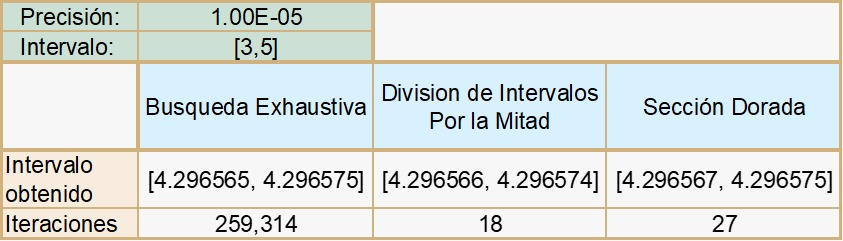
\includegraphics[width = 0.7\textwidth]{figura1}
\end{figure}

\newpage
\subsection*{Codigo Fuente}
\subsubsection{Búsqueda Exhaustiva}
\begin{lstlisting}
	format long
	clc;
	clear;
	global fcalls
	
	%Ingresar los limites y el numero de iteraciones
	a = input('Limite inferior: ');
	b = input('Limite superior: ');
	e = input('Tolerancia: ');
	
	
	%Calcular la longitud del intervalo y el numero de iteraciones
	L = abs(b-a);
	n = 2*(L/e);
	
	%Definir
	deltax=(b-a)/n;
	x1=a;
	x2=x1+deltax;
	x3=x2+deltax;
	contador=1;
	fcalls = 0;
	l1 = L;
	
	%Ciclo para iterar mientras el numero de veces solicitadas
	while (l1 > e)
		if (f(x1)>=f(x2))&&(f(x2)<=f(x3))
			fprintf('El minimo se encuentra en el intervalo (%4.6f,%4.6f)\n',x1,x3);
			%Si se cumple esta condicion, no se ejecuta el resto del while
			break;
		else
			x1=x2;
			x2=x3;
			x3=x3+deltax;
				if x3>b
					fprintf('El optimo es %4.2f o %4.2f\n',a,b);
				%Si se cumple esta condicion, no se ejecuta el resto del while
				break;
				end
		end
		contador=contador+1;
		l1 = abs(x3-x1);
	end
	
	fprintf('Numero de iteraciones: %d\n',contador);
	valor_optimo=(x1+x3)/2;
	evaluacion=f(valor_optimo);
	
	fprintf(['Valor optimo: %4.6f \n ' ...
		'Funcion evaluada en el valor optimo: %4.6f'], valor_optimo, evaluacion);
	  
	fprintf('Numero de llamadas a la funcion: %d\n',fcalls);
	
	function y = f(x)
		global fcalls
		y = sin(x)/(1+x^2);
		fcalls = fcalls + 1;
	end
	\end{lstlisting}
\subsubsection{División de Intervalos}
\begin{lstlisting}
	format long
	clc;
	clear;
	global fcalls
	
	%Ingresar los limites y el numero de iteraciones
	a = input('Limite inferior: ');
	b = input('Limite superior: ');
	e = input('Tolerancia: ');
	
	%Calcular la longitud del intervalo y el numero de iteraciones
	L = abs(b - a);
	xm = (a+b)/2;
	
	fcalls = 0;
	iter = 1;
	
	%Ciclo para repetir mientras no se alcance la precision
	while L>e
		x1 = a + L/4;
		x2 = b - L/4;
		if f(x1) < f(xm)
			b = xm;
			xm = x1;
		elseif f(x2) < f(xm)
			a = xm;
			xm = x2;
		else
			a = x1;
			b = x2;
		end
		%Nueva distancia
		L = abs(b - a);
		fprintf('Iteracion %d:  Intervalo: (%f, %f)  Valor:  %f\n',iter,a,b,xm);
		disp(L);
			iter = iter +1;
	end
	
	valor_optimo=(a+b)/2;
	evaluacion=f(valor_optimo);
	
	fprintf(['Valor optimo: %4.7f \n ' ...
		'Funcion evaluada en el valor optimo: %4.8f\n'], valor_optimo, evaluacion);
	fprintf('Numero de llamadas a la funcion: %d\n',fcalls);
	
	
	function y = f(x)
		global fcalls
		y = sin(x)/(1+x^2);
		fcalls = fcalls + 1;
	end
	\end{lstlisting}
\subsubsection{Sección Dorada}
\begin{lstlisting}
	clc;
	clear;
	global fcalls

	%Ingresar los limites y el numero de iteraciones
	a = input('Limite inferior: ');
	b = input('Limite superior: ');
	e = input('Tolerancia: ');

	%Definir
	t = (-1+sqrt(5))/2;
	L = b - a;
	x1 = b - t*L;
	x2 = a + t*L;
	n = 1;
	fcalls = 0;
	fprintf('\n%d: [%d,%d], L = %d, x1 = %d, x2 = %d\nf(x1) = %d, f(x2) = %d\n',n,a,b,L,x1,x2,f(x1),f(x2))

	%Ciclo para repetir mientras no se alcance la precision
	while L>e
		if f(x1) < f(x2)
			b = x2;
			x2 = x1;
			L = b - a;
			x1 = b - t*L;
		else
			a = x1;
			x1 = x2;
			L = b - a;
			x2 = a + t*L;
		end
		n = n + 1;
		fprintf('\nIteracion %d: [%d,%d], L = %d, x1 = %d, x2 = %d\nf(x1) = %d, f(x2) = %d\n',n,a,b,L,x1,x2,f(x1),f(x2))
	end

	valor_optimo=(a+b)/2;
	evaluacion=f(valor_optimo);

	fprintf(['Valor optimo: %4.6f \n ' ...
		'Funcion evaluada en el valor optimo: %4.6f'], valor_optimo, evaluacion);

	fprintf('\nLlamadas a la funcion: %d\n',fcalls)

	function y = f(x)
		global fcalls
		y = sin(x)/(1+x^2);
		fcalls = fcalls + 1;
	end
\end{lstlisting}

\subsection[Ejercicio 2]{}
Ejecutar sus programas del inciso anterior, y reportar los resultados con una
precisión de $0.05$. El reporte debe incluir la salida de cada programa, o una
parte de ella que muestre que el programa hace las iteraciones correctamente (p.ej. los valores de $L$ o cómo se va reduciendo el intervalo). En particular, debe
reportarse el valor óptimo encontrado $(x^* y f(x^*))$ como el punto medio del
intervalo final.

\begin{figure}[H]
    \centering
    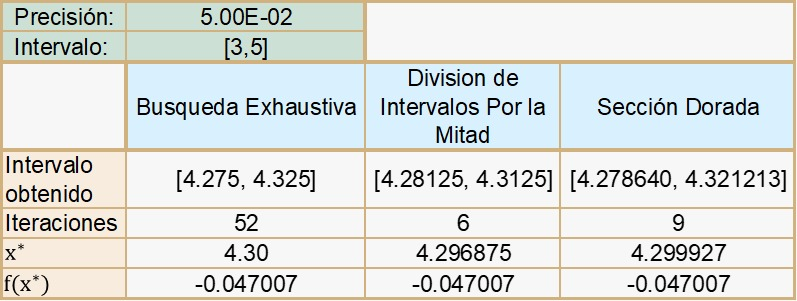
\includegraphics[width = 0.7\textwidth]{figura2}
\end{figure}


\subsection[Ejercicio 3]{}
Ejecutar los programas anteriores para los siguientes valores de intervalos: [3,5], [3.5,5.5], [4,6], [-8,-6], [-8.5,-6.5], [-7,-9],[-2,0],[-1.5,0.5],[-1.3,0.7],[1,6]. Hacer una tabla, con la cantidad de veces que se calculó (i) la
función objetivo, y (ii) el número de iteraciones en cada caso (i.e. (a)
búsqueda exhaustiva, (b) div. de intervalos por la mitad, y (c) sección
dorada) usando cada intervalo. Considere un tamaño de $10^{-12}$ para el intervalo
final. Presentar en su reporte dicha tabla con los valores promedio y la
desviación estándar sobre los 10 valores (de número de iteraciones y llamadas
a la función objetivo) en cada caso. Presentar en su reporte dicha tabla con
los valores promedio y la desviación estándar sobre los 10 valores en cada caso. Ejemplo: escribir en X el número de evaluaciones de $f$ para
cada caso:



\begin{figure}[H]
    \centering
    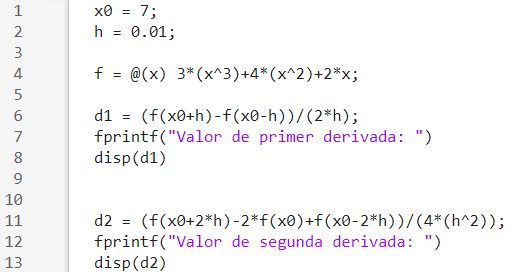
\includegraphics[width = 0.9\textwidth]{figura3}
\end{figure}
\begin{figure}[H]
    \centering
    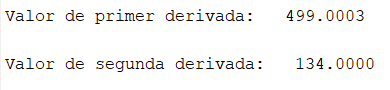
\includegraphics[width = 0.9\textwidth]{figura4}
\end{figure}
\begin{figure}[H]
    \centering
    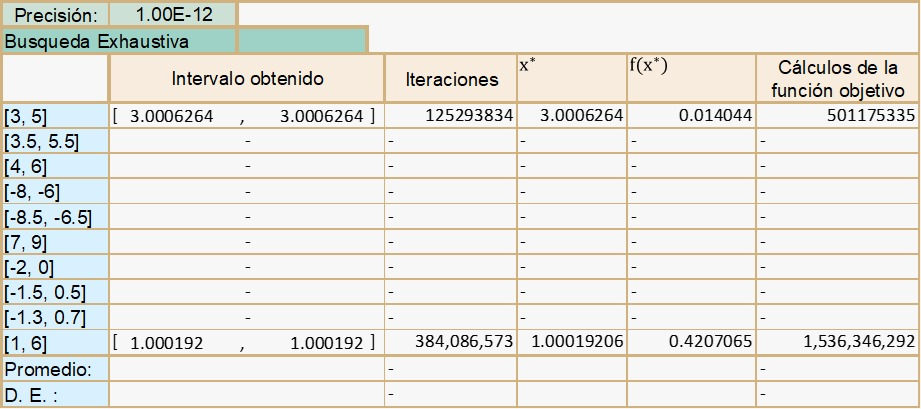
\includegraphics[width = 0.9\textwidth]{figura5}
\end{figure}

\subsection[Conclusiones]{}
Escriba sus conclusiones para toda esta sección. Verifique si los experimentos
son consistentes con las fórmulas que obtuvo en la sección 1.3.

\textit{De las ejecuciones anteriores, vemos que el método de División de intervalos por la mitad es mejor, ya que obtenemos la misma precisión con menos iteraciones y menos evaluaciones de la función y, una vez más, queda descartado el método de búsqueda exhaustiva.
Cabe mencionar que se empleó Arch como SO, lo que aceleró el proceso de iteraciones, sin embargo, por cada intervalo se tardó aproximadamente unos 40 minutos, resultando bastante ineficiente.
Por otra parte, vemos que los resultados obtenidos en cuanto al número de iteraciones son congruentes con las fórmulas de la sección 1.3
En el método de búsqueda exhaustiva la eficacia de las fórmulas se había demostrado previamente. 
Para el método de división de intervalos, para los primeros 9 intervalos, todos con una longitud de 2, el valor resultante de n fue de 40.8631 mientras que para el último intervalo, el valor resultante fue de 42.1850. Aplicando la función parte entera (dado que no se pueden considerar iteraciones que no sean números enteros), los valores concuerdan respectivamente con 41 y 43.
Para el método de Sección Dorada, en los primeros 9 intervalos, todos con una longitud de 2, el valor resultante de n fue de 59.8601 mientras que para el último intervalo, el valor resultante fue de 61.76. Aplicando la función parte entera (dado que no se pueden considerar iteraciones que no sean números enteros), los valores concuerdan respectivamente con 60 y 62.}


\chapter{Bibliografía}

\begin{itemize}
    \item n.d. UNIDAD Nº4 Métodos matemáticos de optimización no restringida Búsqueda unidimensional. [ebook] p.8. Available at: \url{<https://www.fio.unicen.edu.ar/usuario/cgely/q13-0/Apuntes/unidad4.pdf>} [Accessed 8 September 2022].
    \item Coello Coello, C., 2008. Optimización en Ingeniería Clase 2. [ebook] Ciudad de México. Available at: \url{<http://delta.cs.cinvestav.mx/~ccoello/optimizacion/clase2-opt-2008.pdf>} [Accessed 8 September 2022].
    \item Coello Coello, C., 2009. Optimización en Ingeniería Clase 3. [ebook] Ciudad de México. Available at: \url{<http://delta.cs.cinvestav.mx/~ccoello/optimizacion/clase3-opt-2009.pdf>} [Accessed 8 September 2022].
\end{itemize}

\end{document}